\documentclass{beamer}

\usepackage{graphicx, subfigure}
\usepackage{amsmath}


% \usepackage{beamerthemesplit} // Activate for custom appearance

\title{\color{blue} The Street Score project and Visual Perceptions of Safety: Scope for Improvement? }
\subtitle{\color{magenta}Knowledge Lab Team Presentation}
\author{ Nandana Sengupta}
\date{\color{blue}\today}


\begin{document}


\frame{\titlepage}
\frame{\titlepage}

\frame{
\frametitle{The Street Score Project}
\begin{itemize} \small

\item<2-> MIT Media Lab Project
\item<3-> Generating database of visual perceptions of safety/uniqueness etc
\item<3-> 
\includegraphics[width = 0.75\textwidth]{streetscore}
\item<4-> Participants shown \textbf{random} pairs of images
\item<5-> {\color{magenta}Main application:} ranking of neighborhoods/ cities.
\item<6-> Ranking methodologies -- Borda Score (win ratios), Microsoft True Skill Algorithm (Online gaming)
\item<7-> {\color{magenta}Cities in dataset:} Boston, NYC, Linz, Salzburg
\item<8-> Number of images: 4109 , Number of participants: 7872 , Number of comparisons: 208738. 

\end{itemize}


}






\frame{
\frametitle{Limitations and Scope for Improvements}
\begin{itemize} \small

\item<1-> {\color{magenta} Limitations}

\begin{itemize} \small
\item<2->  Images taken from Google Street View -- represents the way cities look from a car

\item<3->  Images are typically from early mornings -- less traffic, people, shops closed

\item<4-> Data collection methodology random -- not taking advantage of similarity in images or participants

\item<5->  Sparsity of win-loss matrix, sampling of locations

\item<6-> Prediction accuracy

\end{itemize}


\item<1-> \color{magenta}{Scope for Improvements}

\begin{itemize}\small

\item<8-> Compare prediction accuracy of different ranking methods: Borda, TrueSkill, SVM, SVM with features.

\begin{itemize} \small
\item<9-> Might require clustering data due to sparsity of observations.
\item<10-> Extraction of features: visual and demographic.
\end{itemize}


\item<11-> Use Active Learning techniques for collecting data.

\begin{itemize} \small
\item<12-> Might require setting up a new survey 
\end{itemize}

\end{itemize}

\end{itemize}


}





\frame{
\frametitle{Feature Extraction}
\begin{itemize} \small


\item<1-> {\color{magenta}Visual Feature Extraction }

\begin{itemize} \small
\item<2-> MIT's Places CNN (Convolution Neural Networks)

\item<3-> Deep Learning Software, open source

\item<4-> Scene Recognition: 205 scene categories eg, residential, highway, apartments etc.

\item<5-> User Input: Raw Image
\end{itemize}

\item<1-> {\color{magenta}Demographic Feature Extraction }

\begin{itemize} \small
\item<6-> US Census Data and American Community Survey Database 

\item<7-> Demographic characteristics by region, eg, average income, educational levels, racial distribution etc 

\item<8-> User Input: Latitude and Longitude
\end{itemize}

\end{itemize}


}




\frame{
\frametitle{Feature Extraction using Deep Learning Software}

\begin{center}

\textbf{Top 3 Predictors:} (office building, apartment building, hospital ) \\


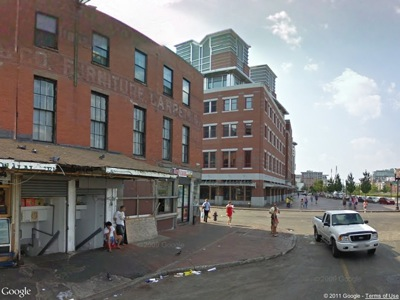
\includegraphics[width = 0.4\textwidth]{id_1_400_300.jpg}

\textbf{Top 3 Predictors:}(yard, residential neighborhood,  driveway) \\

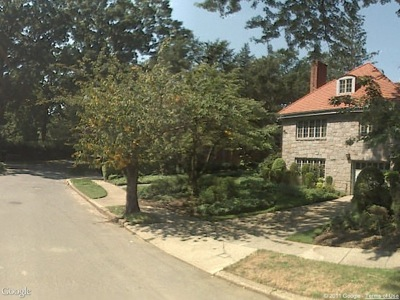
\includegraphics[width = 0.4\textwidth]{id_272_400_300.jpg}



\end{center}



}



\frame{
\frametitle{Feature Extraction: distribution across physical area}


\begin{center}
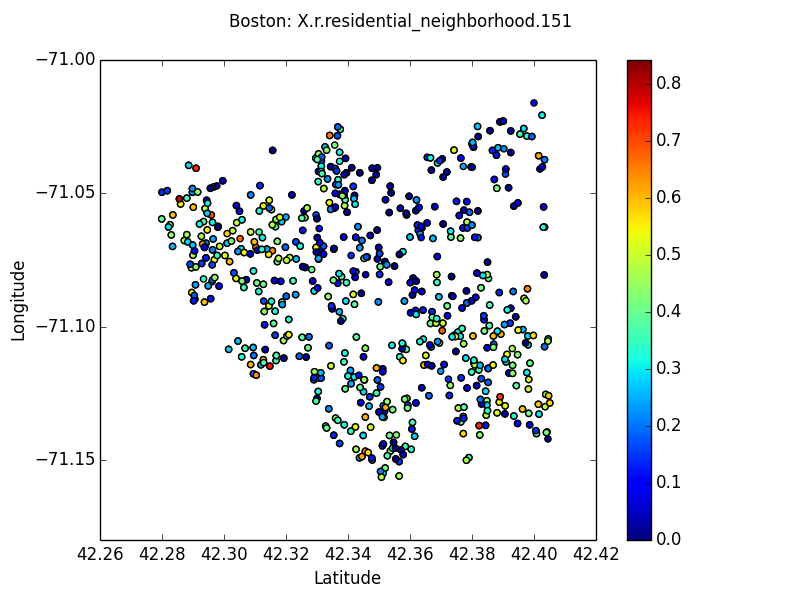
\includegraphics[width = 0.525\textwidth]{bosres}

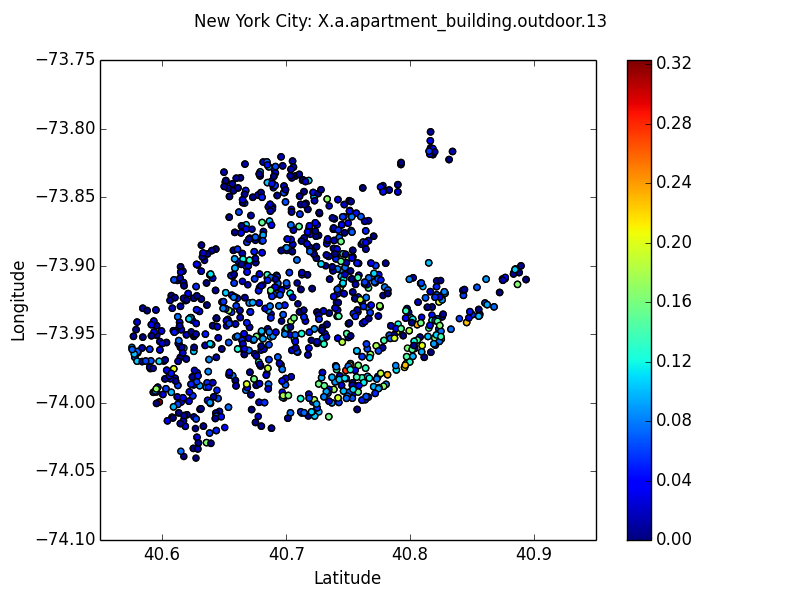
\includegraphics[width = 0.525\textwidth]{nycapart}

\end{center}




}





\frame{
\frametitle{Digging Deeper into the Data}
\begin{itemize} \small

\item<2->  Current number of comparisons svm training difficult 

\item<3-> Multiple images at the exact location

\item<4-> Image comparisons across cities

\item<5-> {\color{magenta}We focused on a single city Boston}

\begin{itemize} \small
\item<6-> 1237 images from 635 unique locations

\item<7->  More sparse than overall matrix but still not enough observations for consistent ranking

\item<8->  Divided images into 100 clusters uaing k-means clustering 

\item<9-> Features for each cluster is the weighted average of member images
\end{itemize}
\item<10> Now ready to run different ranking techniques

\end{itemize}


}



\frame{
\frametitle{Clustered Data for Boston: Top 30 clusters}



\begin{center}

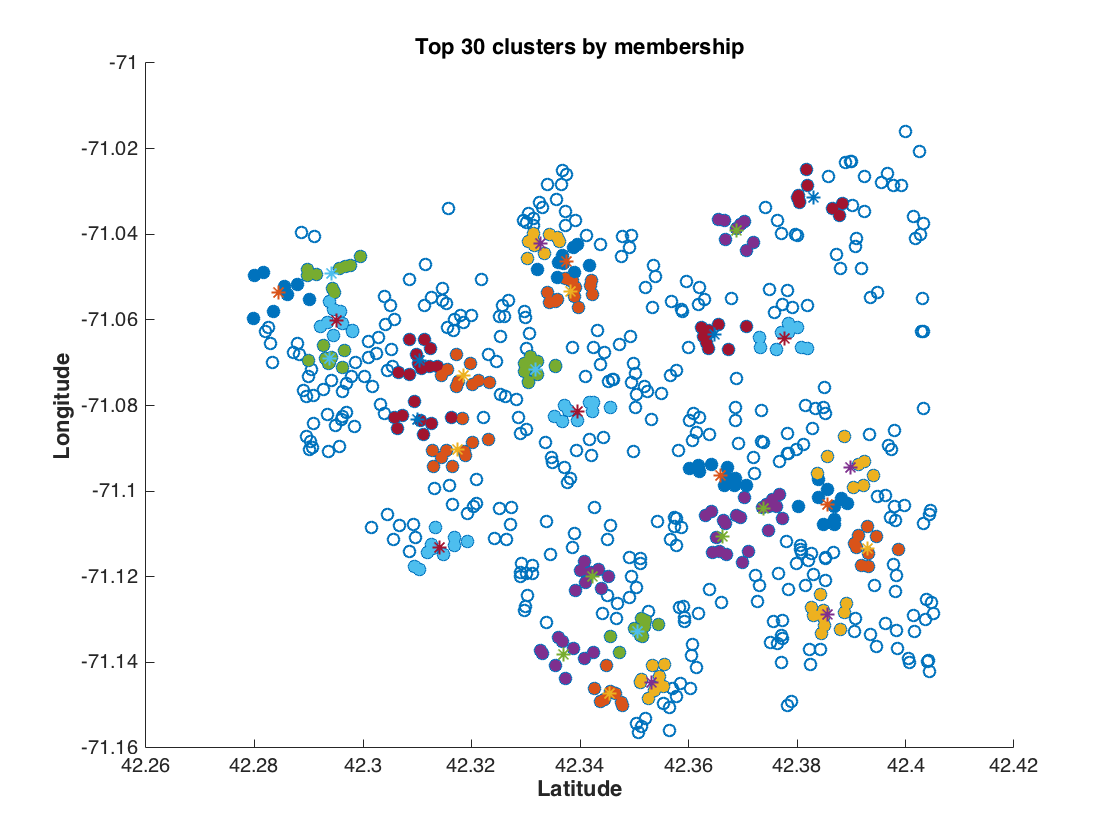
\includegraphics[width = 0.75 \textwidth]{boston_clusters}

\end{center}






}


\frame{
\frametitle{Next Steps}
\begin{itemize}

\item<2-> Run prediction models on clustered data.
\item<3-> Include demographic features in prediction model.
\item<4-> Depending on results, consider possibilities for applying active learning techniques for future data collection.







\end{itemize}


}



\frame{
\centering 
\color{magenta}
Thanks!
}



\end{document}

